\documentclass[11pt]{article}
\usepackage{mypackages}
\begin{document}

\maketitle

\section{Introduction}

The natural way of learning is through repeatedly solving the same
task over and over again, each time observing the result and connecting
actions with outcomes.

Using these principles in a machine learning approach
we can find the sequence of actions that provide the best outcome - a technique known as
\textit{reinforcement learning}.

The goal of this project is to investigate the advantages of asynchronous reinforcement
learning in an advanced setting - playing Atari 2600 games\cite{openAIEnvs}.
Playing an Atari game can be seen as task that is solved by obtaining 
a high score.

This means solving a task consists of being in a certain state and making a decision,
which leads to a new state with a new set of decisions to be made, until
a terminal state is reached.
The terminal state is reached when there are no more decisions to be made
and the task is finished.
Thus a task can be seen as a \textit{decision tree}, with actions connecting states to future states.
%%%%%% Task decision tree
\begin{figure}[H]
    \centering
    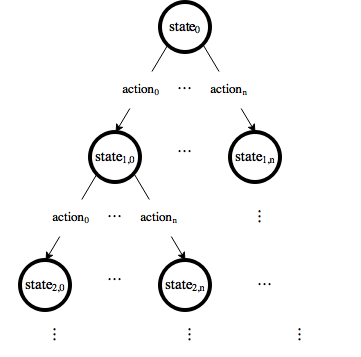
\includegraphics[scale=0.5]{include/decision_tree.png}
    \caption{A decision tree for solving a task.}
    \label{fig:dec_tree}
\end{figure}

In a typical reinforcement learning setting we try to solve a problem
by moving downwards through the decision tree until a terminal state is reached.
The result of taking this exact path is then
taken into account the next time the algorithm tries to solve this problem.

\subsection{Inspiration}

In December 2013 the DeepMind Technologies team published an article
describing an approach to learning from a high dimensional sensory input -
frames from an Atari environment -
using deep reinforcement learning\cite{dqn}.
With a combination of convolutional nerual networks (CNN) and
the reinforcement learning method Q-learning\cite{RLbook} - an approach they
dubbed \textit{Deep Q-Networks} (DQN) - they
presented results proving that it was possible to learn how to play Atari
2600 games at a superhuman level.

Previous reinforcement learning methods haven't been able to succeed at learning to play
advanced games, but the combination of neural networks and
reinforcement learning have made it possible.

A problem that presents itself when a program is learning to play an advanced 
game is that the amount of time and computational resources it takes to train
the algorithm are high.

%As a way to lower the time of training the traditional reinforcement
%learning algorithm can be implemented to do asynchronous training.
%This way the algorithm can take advantage of modern GPUs since
%they are able to execute instructions in parallel\cite{gpu_stuff}.
%Learning asynchronously in this way seems straight forward in deep
%reinforcement learning, since deep neural networks can be optimised
%for GPU usage.

One way to train asynchronously is to run multiple instances of threads on a single
CPU.
Most modern CPUs consists of multiple cores which means it is possible to have a thread
running on each core without taking up resources from each other.
The advantage of asynchronous learning is that multiple different paths
can be explored simultanously, which means that learning can happen at
a higher pace.

An example of asynchronous reinforcement learning was presented by the
Google DeepMind team collaborating with the Montreal Institue for Learning
Algorithms (MILA) in an article from June 2016, where multiple 
reinforcement learning methods were implemented to take advantage of
asynchronous learning\cite{a3c}.

One of the algorithms that were implemented asynchronously
was \textit{advantage actor-critic} (A3C).
This is algorithm that we will use as a benchmark for
comparisons with different amounts of threads.

\subsection{Methods}

In their first succesful attempt at learning to play Atari games using
reinforcement learning the Google deepmind team ran into problems with
the stability of their DQN-algorithm\cite{dqn} - they simply weren't able
to make their algorithm consistently produce satisfactory results.

However, in their next article they adressed their stability problem
and came up with a new algorithm based on the actor-critic method
that takes advantage of asynchronous learning.

With the results of the A3C algorithm in mind\cite{a3c}, the scope of the project we present in
this paper will be to implement the actor-critic algortihm\cite{RLbook}
with a deep learning approach and extend it to exploit the benefits
of asynchronous learning.
%%%% Dette skal kun med hvis vi ikke kan gøre vores eget trådet
%However, due to the time limitations of the project, we will focus on
%the implementation of the actor-critic algorithm and only alter
%an already existing implementation of the a3c method.
%%%%

%In order to test the performance and stability of the actor-critic
%method, we will be using learning environments provided by OpenAI
%gym\cite{openAI} - an open source project which aims at providing
%a simple interface to a collection of reinforcement learning tasks.
%This collection contains a lot of Atari 2600 environments, which we will
%use to compare our results to those presented in \cite{a3c}.

%The main focus of this project is the stability of reinforcement learning
%tasks and how asynchronous learning can be used to achieve better
%stabiliyty.
%We will be presenting the results of the actor-critic method used on a
%simpler task than the Atari environments - the cartpole problem
%\cite{cart_pole} - and then compare an asynchronous approach to the
%results of the DQN-method\cite{dqn} as well as the a3c
%algorithm\cite{a3c}.

%In the remainder of the paper we present and review the reinforcement
%learning environments in the Open AI gym collection and examine the
%theory behind the reinforcement learning methods that will be used -
%i.e. the actor-critic algorithm.
%Furthermore, results of the actor-critic approach to solving the cart-pole
%problem as well as the comparison between our asynchronous approach and
%the one produced by the Google Deepmind team are given.
%Lastly a discussion of these results and the stability problem as a whole
%is presented as well as ideas for further work.

%\printbibliography
%\bibliography{citations}
%\bibliographystyle{plain}
\end{document}
